% !Mode:: "TeX:UTF-8"
\chapter{面向博物馆学习的对话式数字人系统设计}

\section{系统目标分析}
基于第三章提出的 CCEG 框架,本文将系统设计目标确定为三层结构。第一层是学习目标,即提升观众对展品内容的理解深度与记忆稳定性;第二层是交互目标,即支持多轮连续会话并降低提问成本;第三层是表达目标,即通过具身化多模态输出增强重点感知。三层目标共同构成系统设计的评价基线。

在应用层面,系统面向两类典型场景:其一是馆内实时导览,强调响应速度和路径连续性;其二是线上学习导览,强调内容组织和解释完整性。虽然场景不同,但其核心设计约束一致,即系统必须在每一轮交互中同时回答“讲什么、怎么讲、为何现在讲”。

\section{对话式导览设计}
对话式导览设计首先解决知识组织问题。本文将展品知识组织为分层叙事单元,确保系统在首轮回答中提供可理解概览,在后续交互中逐步展开背景解释与跨对象关联。此种设计避免了传统导览“开场过载”现象,使用户能够按自身节奏推进学习。

其次,对话设计强调问题链构建。系统在回答当前问题后,会基于用户意图和导览阶段生成下一步可探索方向,但该引导不以命令式形式呈现,而以“可选追问”方式嵌入自然语言表达。由此,用户既保有路径自主性,又能获得结构化学习支持。

最后,对话设计引入节奏控制机制。对于概念密集段落,系统自动缩短句群并增加停顿提示;对于情境切换段落,系统通过总结句完成语义收束,减少用户在主题跳转时的认知断裂。这一机制使对话从“回答机器”转向“学习组织器”。

\section{导览情境理解设计}
导览情境理解是系统持续有效运行的关键。本文将情境状态建模为一个动态更新对象,包含用户兴趣线索、当前展区信息、历史会话摘要与待解释主题四类核心字段。系统每轮会话都会对该对象进行增量更新,并在下一轮决策时调用。

在策略层,情境理解主要发挥两类作用。一类是难度调节作用,即根据用户问题深度决定回答层级;另一类是路径维持作用,即在多轮交互中保持主题一致并控制切换节奏。当系统检测到用户进入探索型提问阶段时,会提高比较解释比例;当系统检测到用户出现重复提问时,会优先执行归纳性回答并补充缺失背景。

通过上述机制,情境理解不再停留在“记住历史文本”的浅层上下文管理,而成为导览行为的决策中枢。这也是 CCEG 框架区别于一般对话系统的重要特征。

\section{多模态具身引导设计}
多模态具身引导设计围绕“表达为理解服务”展开。系统在生成文本后先进行语义标注,再映射到语音和行为参数。关键术语对应语音重音与轻量强调动作,空间对象对应指向动作与视线移动,话题过渡对应停顿和表情回收。通过这种语义驱动方式,系统可在不增加用户负担的前提下强化重点信息可见性。

角色设定方面,本文将数字人定位为“学习引导者”而非“表演角色”。其语言风格强调准确、温和、可追问,避免过度人格化导致的信息失焦。表达节奏方面,系统对动作频率、表情幅度和语速变化设置上限阈值,以防出现形式干扰内容的问题。

图\ref{fig-prototype-ui}展示了开题阶段原型界面形态。可以看到,界面设计将角色呈现、对话输入和导览情境区并置,使用户能够在同一视域中同时感知“谁在讲、讲什么、讲到哪里”。

\begin{figure}[htbp]
    \centering
    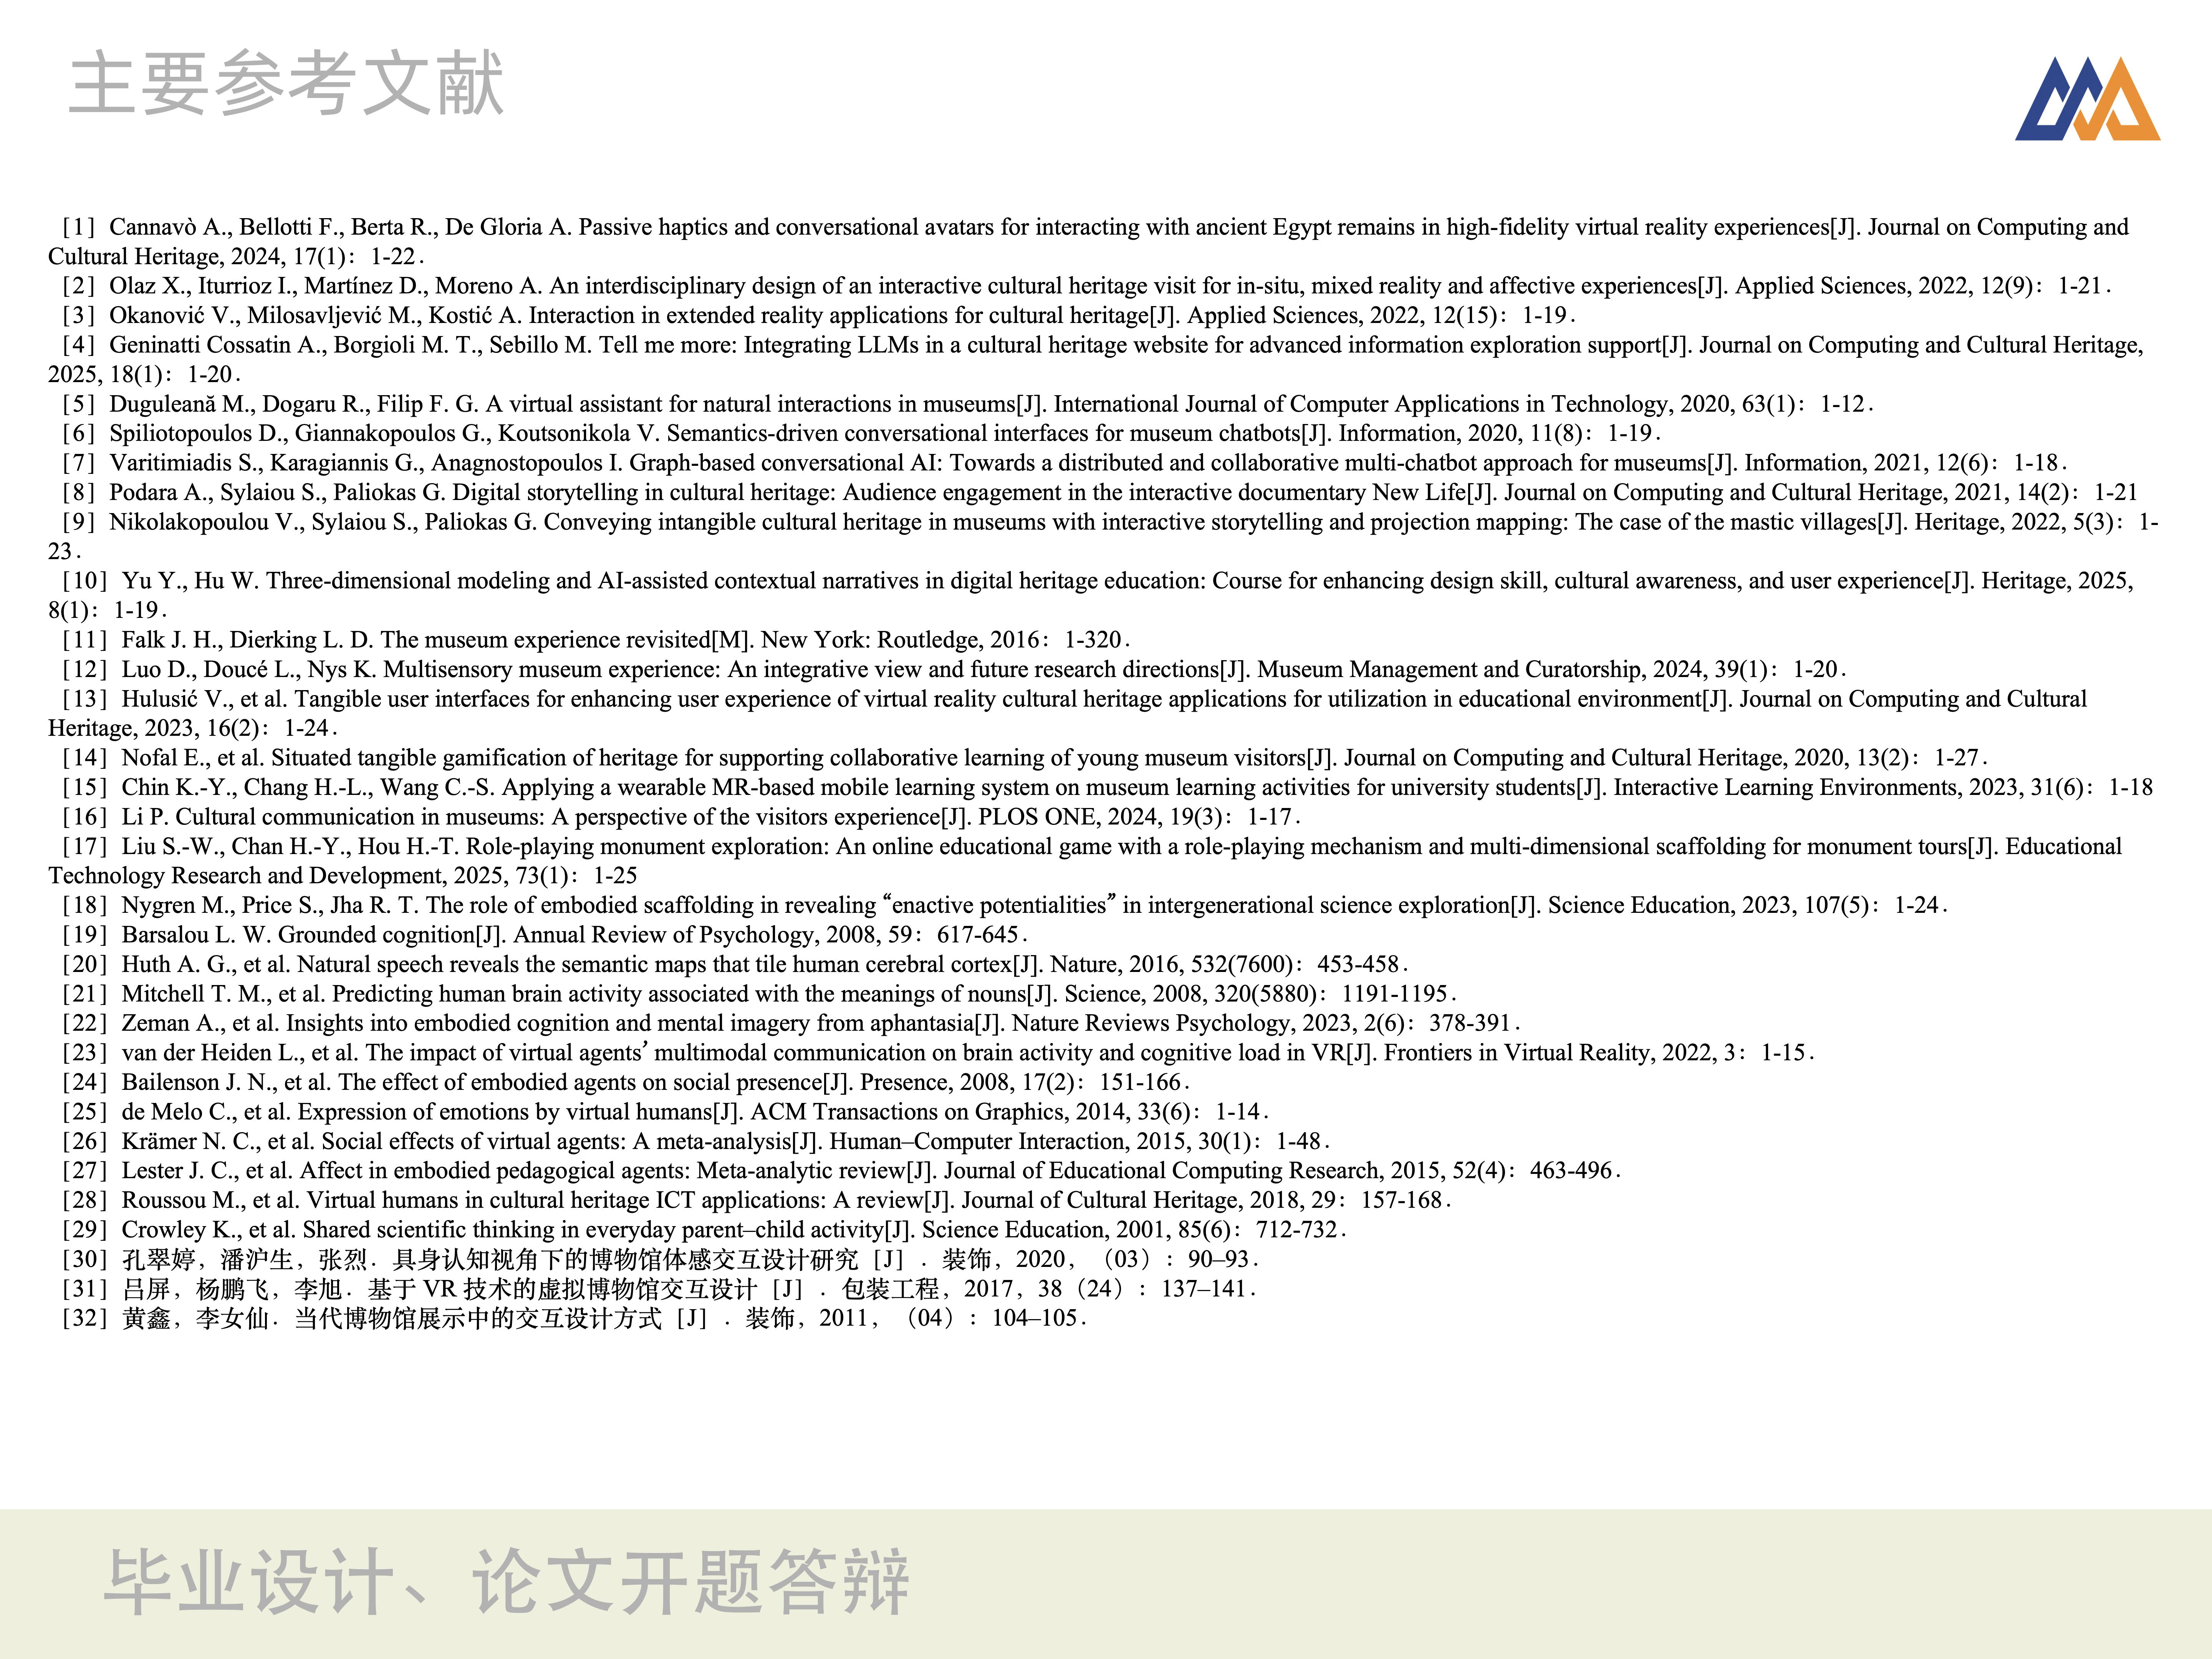
\includegraphics[width=0.95\textwidth]{figure/opening/opening-011.png}
    \caption{对话式数字人导览原型界面(来源:开题报告)}
    \label{fig-prototype-ui}
\end{figure}

\section{本章小结}
本章将 CCEG 框架转化为系统设计方案,分别从目标分析、对话设计、情境理解和具身引导四个层面给出实现路径。研究表明,只有在设计阶段就建立跨模块协同约束,数字人导览系统才能在真实博物馆学习场景中保持连续、稳定且可解释的引导能力。

\section{关键交互场景的设计推演}

\subsection{首次进入场景的引导推演}
首次进入是导览体验建立心智模型的关键阶段。若开场信息过多,用户会迅速产生负担;若开场信息过少,用户又难以确定探索方向。本文在该场景中采用“轻量开场+问题引导”策略:系统先用简短语言说明当前展区主题与可探索方向,再通过一到两个低门槛问题激活用户参与。该策略既提供必要背景,又保留足够交互空间。

\subsection{深度追问场景的推演}
当用户进入深度追问阶段时,系统需从概览解释转向结构化分析。本文设计中,系统会在回答后显式连接前序问题,说明本轮解释与前文关系,帮助用户形成连续知识链。对于跨展品比较问题,系统优先给出比较维度,再逐项展开,避免直接堆砌结论造成理解困难。

\subsection{主题跳转场景的推演}
在真实参观中,用户主题跳转频繁且不可预测。若系统不进行阶段收束就直接跳转,容易导致会话失序。本文在主题跳转场景中设置“过渡总结”机制,即先用一句话归纳已讨论内容,再进入新主题解释。该机制可显著降低认知突变感,是情境连续性的关键设计点。

\section{设计约束与质量控制}
系统设计不仅关注功能完整,也关注质量可控。本文在设计阶段建立三类质量约束:语义约束、节奏约束与一致性约束。语义约束保证回答可追溯且不越界;节奏约束保证输出长度与停顿合理;一致性约束保证语言、动作和表情服务同一导览目标。通过这些约束,系统可在原型阶段即形成可验证的质量边界,为后续实现和评估提供基础。
